%%% approaches.tex: -*- LaTeX -*-  DESCRIPTIVE TEXT.
%%%
%%% Copyright (c) 2017 Brian J. Fox & Orchid Labs, Inc.
%%% Author: Brian J. Fox (bfox@meshlabs.org)
%%% Author: A truckload of others
%%% Birthdate: Tue Oct 10 12:01:02 2017.

\subsection*{Unprotected Internet Access}

Users who access the Internet without protection provide their
complete browsing history and website use to their ISP, who can then share or sell that data.

\subsection*{Virtual Private Networking (VPN) Services}

Virtual Private Networks (VPNs) use encryption to securely transport a
VPN subscriber's traffic across a larger insecure network. Once the
VPN has received the traffic, it is decrypted and retransmitted across
a different large insecure network. The retransmission can assist
users in circumventing access restrictions imposed by websites, and to
a lesser extent, reduce the tracking of their website browsing
habits. Encryption prevents the user's ISP from seeing their traffic,
thereby preventing monitoring attacks. This is accomplished by making
the VPN a new ISP for the user.  Any attack an ISP could previously
perform can easily be performed by the VPN provider.

VPN users should not assume their VPN provider is trustworthy. Although VPN service providers face more competition
than ISPs, they ultimately draw talent from the same sources, and have
similar bandwidth-for-cash-type business models. It is unlikely that
VPN providers will not fall prey to the same incentives which led the
user to not trust their ISP. Additionally, the re-use of IP addresses
for relaying traffic in VPN setups enables relative ease in blocking
their use by commercial websites\cite{13}.

\subsection*{Tor}

Tor\cite{TOR} is a free software project famous for introducing the
idea of \emph{Onion Routing} to a wider audience. In this system, users
download a global list of relays and exit nodes, randomly select from
that list, and form \emph{onion routes} from their selection. Onion
routes are an ordered list of relays; packets sent along an onion
route are encrypted for each peer in turn, ensuring that each node
must have received a packet enroute for it to be understood by the
exit node. The result is that unless several nodes are compromised or
run by the same user, no two relays know both who sent 
a packet and where it went.

\begin{figure}[htpb]
  \centering
  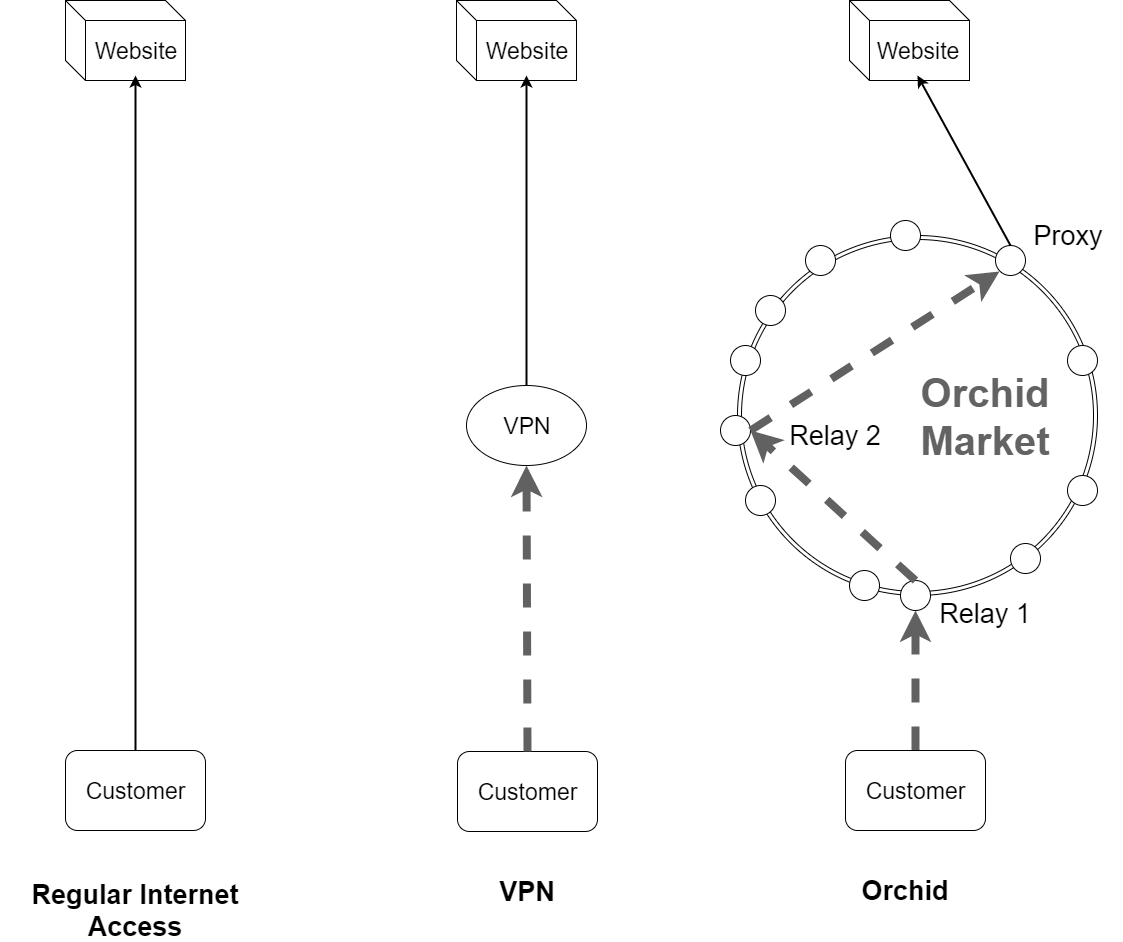
\includegraphics[width = 400pt]{overview}
  \caption{Direct connection, VPN connection, Orchid connection}
\end{figure}

%% @saurik: ref on Dingledine knowing ~75% of relay operators personally?

%% \subsection{Tor with Incentives} ?

%% \subsection{I2P} ?

%% I2P is billed as a “next generation” onion router. It is primarily
%% focused on communication internal to the network.

%% \subsection{Mixmaster, Mixminion, and other Chaumian relay schemes} ?
